\documentclass[11pt,a4paper]{article}
\usepackage[T1]{fontenc}
\usepackage{lmodern,microtype,amsmath,amssymb,booktabs,tabularx,array}
\usepackage{graphicx}
\usepackage[margin=25mm,top=24mm,bottom=26mm]{geometry}
\usepackage[dvipsnames]{xcolor}
\usepackage[colorlinks=true,linkcolor=MidnightBlue,citecolor=MidnightBlue,urlcolor=MidnightBlue,pdftitle={Correlation Actualization Theory: a nonperturbative matrix proposal with observer-dependent layers},pdfauthor={Yohtaro Soga}]{hyperref}
\usepackage{enumitem}
\setlist{nosep}
\newcolumntype{L}[1]{>{\raggedright\arraybackslash}p{#1}}
\renewcommand{\tabularxcolumn}[1]{>{\raggedright\arraybackslash}p{#1}}
\setlength{\emergencystretch}{2em}
\renewcommand{\topfraction}{.90}
\renewcommand{\bottomfraction}{.80}
\renewcommand{\textfraction}{.10}
\renewcommand{\floatpagefraction}{.82}
\newcommand{\Tr}{\operatorname{Tr}}
\newcommand{\id}{\mathbf 1}
\newcommand{\sgn}{\operatorname{sgn}}
\newcommand{\dd}{\mathrm d}
\newcommand{\dof}{\mathcal H}
\newcommand{\source}[2]{\href{#1}{#2}}
\title{\textbf{Correlation Actualization Theory}\\[3pt]\large A nonperturbative matrix proposal with observer-dependent layers}
\author{Yohtaro Soga\\[-1pt]\small Correspondence: \href{mailto:gawakkyu0603@gmail.com}{gawakkyu0603@gmail.com}}
\date{25 November 2026 \quad(Version 4)}
\begin{document}
\maketitle
\begin{abstract}
We propose Correlation Actualization Theory (CAT) as a candidate framework for a theory of everything. Ordinary unitary evolution correlates matter with its surroundings. A gravitational transition can select a layer irreversibly with Born weight; the charge received by an observer can then change which modes carry matter onward. Black-hole infall motivates this rule. The infaller can cross the horizon in finite proper time, while the distant observer's description can end at a surface carrying the infaller's quantum information. Requiring the inward route to disappear exactly leads to a constraint on the allowed states. We give a ten-matrix representation both with a chosen clock and with contacts ordered by material correlations, without an input spacetime metric. The prescription sets no maximum matrix size. Its nonperturbative calculations use complete scattering blocks at specified rank, clock and port. A common-source example realizes the two continuations and permits recovery of a qubit on the exterior histories. A quantum theory connecting the ranks and clock sectors, the widespread formation of the required ports in natural collapse, and information recovery at the evaporation endpoint remain open.
\end{abstract}

\section{A matrix proposal motivated by infall}\label{sec:motivation}
What becomes of a quantum state carried by a falling observer if no signal can ever bring the infaller's final record back to a distant laboratory? Correlation Actualization Theory (CAT) starts with the records these two observers can obtain. It proposes a law for the irreversible selection of layers by gravity, alongside the ordinary unitary dynamics of matter and fields within each layer. Two nearby observers can usually use a common geometry wherever their records agree. The proposal does not require them to have a common spacetime beyond that region.
Suppose A carries a clock, a spin prepared by a colleague, and a small receiver into a large, nearly Schwarzschild black hole. A can relate the spin to nearby matter by ordinary interactions. B stays far outside. Signals received by B from successively deeper on A's trajectory are increasingly delayed and redshifted. Hawking emission is a prediction of quantum fields on a suitable collapsing geometry \cite{hawking,page}. Neither the redshift nor the emission is an observation by B of A being destroyed on the horizon. Classical relativity assigns A a regular crossing. For radial fall from rest at infinity it assigns a proper time \(2r_s/(3c)\) from \(r_s=2GM/c^2\) to the classical singularity. Which description continues to apply when curvature becomes large is a question for the microscopic theory.

Our working hypothesis takes the absence of a possible comparison seriously. A can have an inward continuation. In B's present physical description the hole can instead end at a surface carrying A's correlations. There is then no present B-interior in which a second copy could reside. A later decision by B to fall would create a new sequence of receipts. It supplies no earlier joint observation of the two endpoints. Complementarity already gives the freely falling and exterior observers different operational descriptions \cite{complement,amps}. The extra step here is to specify a physical law that can remove the inward channel in B's evolution while preserving it in A's.

A's matter and the nearby field take part in the same ordinary interactions whichever observer describes them. Giving B less information about those interactions would, on its own, change only B's prediction. We therefore make three physical assumptions. First, ordinary dynamics creates quantum correlations in all the degrees of freedom of the infaller and its surroundings. Second, gravity can separate those correlations into layers and select a material receipt irreversibly with Born weight. The strength of a populated transition enters its scattering amplitude. Third, layers can affect each other's later propagation through the resulting gravitational contact. This coupling can act even when tensor waves do not propagate between layers. Conditioning on the records that make A a local observer can narrow A's own history while leaving many possibilities for A in B's description. No preferred person or location enters the rule.

A density operator within a layer can already be mixed. If the later dynamics is insensitive to which layers were selected, the usual mixed-state predictions suffice. The horizon thought experiment asks for a sharper distinction. A model that leaves even one per cent of B's weight on an inward route still assigns B possible histories with an interior. \textbf{The demand for exact closure in B's description guided our choice of low-energy action.} Section~\ref{sec:ir} compares interactions that suppress a route with a surface constraint that removes the allowed states themselves. Section~\ref{sec:parent} then asks how a matrix action can realize that constraint. The comparisons with other gravity theories and the observational tests follow from these two choices. We use \(c=\hbar=1\) unless units are restored explicitly.

\section{Choosing the low-energy interaction}\label{sec:ir}
\begin{figure}[htbp]
\centering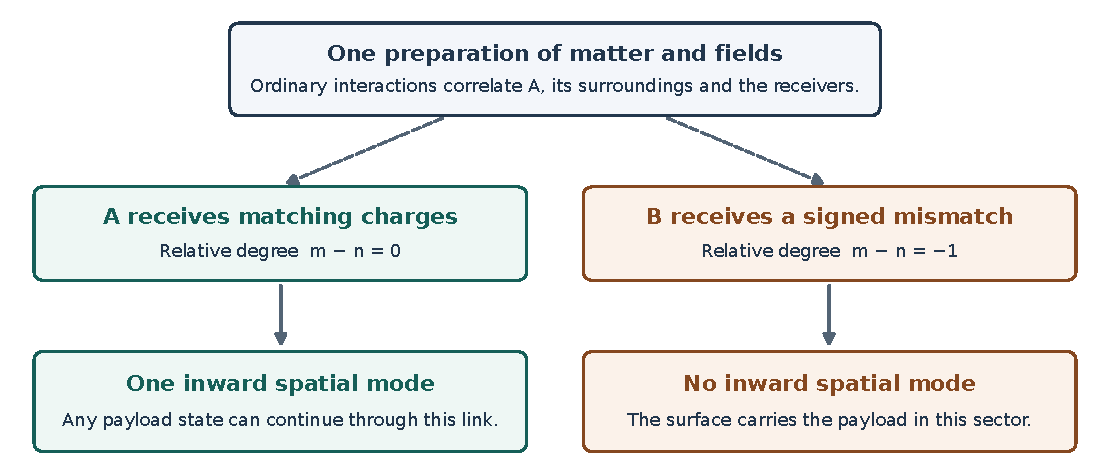
\includegraphics[width=.96\linewidth]{fig-route.pdf}
\caption{The dashed arrows are the outstanding physical preparation problem: can one collapsing source produce these different receipts by their respective deadlines? The solid arrows are consequences of the spherical interface once the indicated charges have arrived. The channel count refers to spatial propagation of an arbitrary carried quantum state.}
\label{fig:routes}
\end{figure}
\subsection{What can carry a difference between layers?}
Ordinary matter can acquire a correlation through the tidal coupling \(H_{\rm tide}=-Q^{ij}{\cal E}_{ij}/2\), where \(Q^{ij}\) is its mass quadrupole and \({\cal E}_{ij}=R_{i0j0}\) in a freely falling material frame (the sign fixes our quadrupole convention). Absorption exchanges real energy and angular momentum. Reversing the field, source and recoil can in principle undo this step. For comparison, gravitational radiation escaping a laboratory or crossing a Killing horizon can itself decohere a superposition accessible to that laboratory \cite{horizondeco}. It is essential to include such ordinary, potentially inaccessible modes when estimating a reversal signal.

We examined two ways for an additional interaction to change a layer. In a mediator description a field \(x\) with quadratic kernel \(D\) couples to a sum of layer sources \(J_h\). Eliminating a Gaussian field in the quadratic action yields a response proportional to \(-\tfrac12\sum_{h,h'}J_h D^{-1}J_{h'}\), with the boundary prescription fixed by the preparation. A causal response calculation uses the retarded kernel on the two branches of the evolution. A direct interaction can give the same static energy. Equal static forces alone cannot decide whether an independent mode propagates. Propagating tensor exchange also faces a sharp test if the layer coordinate is identified with the ordinary M-theory circle: in a parallel, equally charged membrane configuration, the three-form exchange is required along with the metric to give the protected force cancellation \cite{bfss,witten,m2}. Treating every membrane as a different layer and coupling them only by ordinary tensor gravity loses that cancellation.

A second possibility is a \emph{constraint at a received contact}. The word contact denotes a junction that can actually receive the relevant material currents, with compensating charge and recoil present. It can change a continuation even when no tensor wave crosses from one layer to another. A direct instantaneous force between freely controllable, spatially separated laboratories would in general change remote statistics. We restrict the junction to causally available receipts; independent spacelike local instruments must commute at the level of their nonselective operations. If the outcomes are retained, exchanging the order must also preserve the maps for each pair of records and the control applied afterwards. Section~\ref{sec:parent} gives the history law; Sec.~4.1 of the technical supplement works through this stronger condition. A general quantum-gravitational derivation of the full constraint algebra remains open.

\subsection{Why width and dissipation alone do not close the route}
Let \(E\) be the positive effect for an inward continuation at a \emph{fixed} input port, and let \(\rho_A,\rho_B\) be density operators there. If \(\rho_B\geq\lambda\rho_A\) for some \(\lambda>0\), then
\begin{equation}
 p_B=\Tr(E\rho_B)\ \geq\ \lambda\Tr(E\rho_A)=\lambda p_A .
 \label{eq:floor}
\end{equation}
This is the positivity of a trace, related to the usual operator-order comparison of states \cite{datta}. It explains why replacing A's sharp state by a broad ensemble containing it cannot make a common port strictly dark. For \(k\) independently and uniformly drawn \(d\)-valued comparisons, a port that opens on complete agreement retains probability \(d^{-k}\). Ten balanced binary comparisons leave \(1/1024\). A finite integrated decay rate also leaves positive survival. These mechanisms can produce a sharp practical difference. Neither supplies the zero required by B's thought experiment. A different \emph{physical support} for the inward channel can do so.

A broad record need not give the support of A's records at this junction. For example, both descriptions can carry a broad distribution of an absolute integer \(n\) while assigning different, sharp \emph{relative} charges to two received ends. Nor does equality of the two ends reveal which common value was received. The difference can govern propagation and the common value can sharpen A's history without revealing A's unknown payload. In a four-alternative preparation the best guess of a local value rose from \(39\%\) to \(100\%\) after A's receipt, and stayed at \(39\%\) upon B's symmetric receipt. Giving B one further ordering bit raised it to \(43.21\%\). The distinction depends on \emph{all} accessible records, not on coordinate distance alone.

\subsection{The spherical interface}\label{sec:sphere}
Let the lines selected by two material ends over a sphere of directions have degrees \(n\) and \(m\), using the orientation of the receiving surface. An inward field \(Y\) is a section of their comparison line \(L=\mathcal O(m-n)\) over \(\mathbb{CP}^1\). A local multiplier imposes its covariant holomorphic constraint. Schematically the interface contribution is
\begin{equation}
 S_{\partial}=\int_{\Sigma}\! \mathrm{Re}\langle \lambda,\bar\partial_LY\rangle\,
             \dd\mu_{\Sigma},\qquad
 N_{\rm in}=\dim H^0(\mathbb{CP}^1,L)=\max(1+m-n,0).
 \label{eq:route}
\end{equation}
Here \(\lambda\) is a dual-valued multiplier, the pairing includes the surface density, and the count uses the spherical polarized sector. Holomorphic sections of a line bundle on the sphere are classical mathematics \cite{groth}. The physical postulate is that propagation of every component of A through this junction requires such a section. The same constraint has a finite matrix realization: the two coordinate multiplication maps must intertwine. Its \(k\)-th column is a translate of the first, whose support is \(0,\ldots,m-n\). The corresponding finite statements have been formalized and checked in Lean (Appendix~\ref{sec:verification}).

For \(m=n\) one spatial link carries the entire payload, including entanglement with a reference. For \(m=n-1\) there is no inward degree of freedom. In this B-sector the surface and its exterior give the domain of subsequent evolution; an unobserved interior behind an opaque wall would be a different model. Reversing the sign of the mismatch gives two allowed modes. The orientation of a deposited charge is therefore measurable in principle. For this claim the physical angular sphere of the junction carries the holomorphic constraint for each allowed spin and species in the chosen energy band. The sphere of matrix-probe directions determines the signed material index. A nontrivial species bundle or another inward connection can reopen transmission. A finite energetic penalty for violating the constraint only approximates this result. A common distribution over many \(n\)'s preserves exact closure if each occupied B-sector has \(m=n-1\). A nonzero weight in a matched sector reopens it. The zero counts the specified port. Interpreting the entire B-description as exterior only additionally takes this surface to exhaust its possible continuations, or requires closure at every accessible inward port. Closure in one angular patch cannot establish that global statement.

There is an independent restriction from causal propagation. A strictly local surface coinciding with a classical null event horizon cannot first receive information there and then send it to future null infinity along a classical outgoing causal curve. A timelike emitting boundary outside a trapped region, a receding timelike trapping surface, or encoding in exterior modes before the last contact can provide an outgoing channel. A coupling to exterior tidal fields at finite radius is another, radially nonlocal, effective candidate. Our spherical comparison fixes the allowable \emph{inward} modes. The causal surface, emission amplitudes and their time scales must still be supplied by the microscopic solution.

\section{A matrix action for matter, selection and gravitational feedback}\label{sec:parent}
\subsection{Ordinary evolution and the material crossing}
The parent we adopt, Correlation Actualization Theory (CAT), has a reversible part with ten Hermitian matrices \(X^a\), a Majorana--Weyl spinor \(\Psi\), and a target contraction of signature \((9,1)\). In Lorentzian conventions it is
\begin{equation}
 S_0=+\frac{1}{g_0^2}\Tr\left(\frac14[X^a,X^b][X_a,X_b]
             +\frac12\bar\Psi\Gamma^a[X_a,\Psi]\right).
 \label{eq:ikkt}
\end{equation}
We use the IKKT interactions \cite{ikkt} with Hermitian matrices, \(\eta={\rm diag}(-,+,\ldots,+)\) and forward weight \(e^{+iS_0}\). The negative Euclidean contraction of the original matrix integral uses \(e^{-S_E}\). A material clock sector can be represented by \(X^0=-i\partial_\tau+a_0\) on a translation quotient of period \(\beta\), with nine remaining matrices \(X^i(\tau)\). With normalized trace per period \(g_1^2=\beta g_0^2\). The bosonic Lorentzian action in that sector reads
\begin{equation}
 S_{\rm clock}=\frac1{g_1^2}\int\dd\tau\,\mathrm{tr}
 \left\{\tfrac12(D_\tau X^i)^2+\tfrac14[X^i,X^j]^2\right\},
 \label{eq:bfss}
\end{equation}
Indeed \([X^0,X^i]=-iD_\tau X^i\), so contracting both time--space orders gives \(+2(D_\tau X^i)^2\). Writing \(\Pi_i=D_\tau X_i/g_1^2\), the physical bosonic Hamiltonian is \({\rm tr}[g_1^2\Pi_i^2/2-[X_i,X_j]^2/(4g_1^2)]\). On the adjoint singlet sector the connection imposes the Gauss constraint. The supplement spells out the fermion convention, Wick rotation and signed clock tests. The second term has nonpositive trace for Hermitian matrices. This is the usual matrix quantum mechanics under the quotient assumptions \cite{bfss,taylor}. It is the time-based version used for matching to the exterior. The clock period, state and coupling set reference units here. There is no derivation of their measured values from the history law.

To decide which material correlation can write a history, take a material three-plane separated by a gap in the inertia tensor, with its handedness fixed by an oriented material observable. At gaps or orientations that cannot be resolved, this prescription requires further input. A Hermitian spinor probe uses \(D=\sum_I\gamma_I(X_s^I-y^I)\), where \(s\) labels the source block and \(y\) the material probe position in the matrix configuration. In an oriented orthonormal frame define
\begin{equation}
 \chi=-i\gamma_1\gamma_2\gamma_3,\quad
 D_\parallel=\tfrac12(D+\chi D\chi),\quad
 \nu=\tfrac1{16}\Tr\!\left[\chi\,\sgn(D_\parallel)\right].
 \label{eq:index}
\end{equation}
Here the matrix index counts spectral signs on the two gapped sides of a crossing. A receipt is an ordinary absorbed transition with a physically compensated charge. Occupation refers to that transition carrying amplitude. The law actualizes its outgoing charge sector as an irreversible record. The signed fuzzy-sphere receiver in the supplement supplies an explicit handedness observable. This adapts the established matrix membrane index \cite{berenstein}. For the index sectors used here, a gravitationally occupied, isolated crossing of jump \(\Delta\nu\) transports \((q,c)\mapsto(q+\Delta\nu,c-\Delta\nu)\) to a receiving and a compensating port. A reversible level crossing or a charge pump by itself does not supply irreversible selection. The receipt requires a nonzero on-shell transition and an energy source. For a massive receiver initially at rest, raising its rest mass from \(M\) to \(M'\) by absorbing one massless quantum requires \(\omega=(M'^2-M^2)/(2M)\). Source, support and recoil must be included when applying this condition.

\subsection{The action for histories}
Write \({\cal U}_e\) for ordinary evolution and reversible matching through one candidate contact. Let \(P_z\) resolve the deposited, physically distinguishable charge, including an empty outcome. Let \(B_z\) be the isometry accounting for the corresponding physical record and recoil. On a history \(h\), with subnormalized density \(\rho_h\), the forward rule is
\begin{align}
 K_z&=B_zP_z{\cal U}_e,&
 \rho'_{h'}&=\sum_{\Lambda(h,z)=h'}K_z\rho_hK_z^\dagger,&
 \sum_z K_z^\dagger K_z&=\id .
 \label{eq:write}
\end{align}
Selection of \(z\) has probability \(\Tr(K_z\rho_hK_z^\dagger)/\Tr\rho_h\) when \(\Tr\rho_h>0\). A continuous spectrum or a sequence of contacts gives arbitrarily many alternatives. For continuous outcomes the primitive observable is the instrument on a \emph{measurable set}, for instance \(\int_\Delta K_z\rho K_z^\dagger\dd\mu(z)\) when an operator density exists. A single point of zero measure is never assigned a finite probability by a formal delta-function projector. The history is the selected layer or set of layers. A reverse material transfer can discharge a port, and the map \(\Lambda\) may merge later labels. Lost coherences do not follow from reading the present charge alone. The choice of a fundamentally irreversible selection is a postulate beyond ordinary unitary environmental decoherence \cite{luders,relational,tilloy}.

For contact \(e\), \(J_e\) maps the possible payload to the local comparison space and \(d_e\) takes the difference read there. Put \(T_e=d_eJ_e\). The occupation vector \({\bf n}\) counts the physical contacts that are present. With \(S\) the swap of the degenerate inward and surface routes, define
\begin{align}
 C_{\bf n}&=\sum_e n_e T_e^\dagger T_e,&
 P_{\bf n}&=\mathbf 1_{\{0\}}(C_{\bf n}),&
 W_{\bf n}&=P_{\bf n}\otimes\id+(\id-P_{\bf n})\otimes S .
 \label{eq:feedback}
\end{align}
The two routes carry the same payload space. Since the terms in \(C_{\bf n}\) are positive, only an input annihilated by every occupied comparison can continue inwards. Across mutually exclusive material configurations one uses a single operator \(\mathbb W=\sum_{\bf n}|{\bf n}\rangle\langle{\bf n}|\otimes W_{\bf n}\). For diagonal occupation blocks the inward probability is \(\sum_{\bf n}p_{\bf n}{\rm Tr}(P_{\bf n}\rho_{\bf n})\); arbitrarily small weight in a different configuration does not redefine the operator. For an integrable family of positive quadratic forms the condition holds almost everywhere on occupied support, on their common form domain. Pure rescalings of positive strengths cannot change that kernel. A gravitationally received inequality can thus change a later trajectory without allowing ordinary matter to excite a new interlayer gravitational wave directly. Physically distinct layers can participate in a comparison only through the prescribed material junction. Applying \(W\) to unconstrained, externally controllable hidden data would require a separate causality test.

Equations~\eqref{eq:ikkt}, \eqref{eq:index}--\eqref{eq:feedback} specify a \emph{doubled} action: an interval has weight \(e^{iS_0[X_+]-iS_0[X_-]}\); a received crossing inserts the superoperator \(\sum_z K_z\otimes\overline K_z\) with its outgoing charge sectors, and routing inserts \(W\otimes\overline W\). Independent empty intervals have ordinary unitary propagation. This specification as an influence functional and local instruments identifies precisely where the usual closed-system unitarity has been relaxed. A complete channel respects local exchange on the matched port when, for each conserved total generator \(Q\), its spectral projections obey \(\Pi_{\rm out}(\Delta)K_z=K_z\Pi_{\rm in}(\Delta)\), and likewise for routing. This is a stringent condition on an implementation, including four-momentum. Trace preservation alone does not imply it. The explicit experiment in Sec.~\ref{sec:joint} satisfies this condition on a flat energy shell and fixes remote observables for local instruments. This addresses one issue raised for fundamental pure-to-mixed evolution \cite{bps}; a covariant energy balance for arbitrary emergent geometries remains to be obtained.

\paragraph{Which part of a history depends on the observer?}
Fix the matrix rank, a material clock sector and a network of physical contacts. At contact \(e\), let \(L_{e,z}=\mathbb W_e K_{e,z}\) for receipt \(z\); use \(\mathbb W_e=\id\) if no separate routing occurs. The clock orders the contacts. The factors may depend on receipts already available at that port. If \(R_O({\bf z})\) is the part of the record that reaches observer \(O\), its operation on the common preparation \(\rho\) is
\begin{equation}
 \mathcal I^O_r(\rho)=\sum_{R_O({\bf z})=r} L_{\bf z}\rho L_{\bf z}^{\dagger},
 \qquad L_{\bf z}=L_{e_s,z_s}\cdots L_{e_1,z_1}.
 \label{eq:matrixhistory}
\end{equation}
The trace gives the Born weight and normalization gives the conditional state. On this fixed network every fine history occurs once in the sum over \(r\). All observers therefore have the same total channel when the outcomes are discarded. This remains true with adaptive contacts if the operations are complete after each reachable sequence of receipts. The composition of instruments is standard quantum-network theory \cite{networks}.

CAT makes a further physical prescription. Each observer uses the material port reached by that observer's signals, the charge recorded there at the deadline, and the output modes allowed by that charge. A recorded charge controls a subsequent operation even if no one later reads the register. Section~\ref{sec:joint} follows one qubit from a common preparation. On a joint receipt of weight \(0.196608\), A's port admits an inward copy of the \emph{code space}; B's port has zero inward dimension and admits a surface carrier. Each map acts on the one unknown input in its own description. In a common causal region a delivered copy of the same classical receipt must give the same probabilities. The supplement specifies the maps, the accessible observables and the outcome-wise clock-order condition.

\paragraph{Matrix size and the scope of the proposal.}
The ten labels \(a\) in Eq.~\eqref{eq:ikkt} count matrix components; \(N\) is the size of each matrix. CAT fixes neither a highest \(N\) nor a universal number of gravitational contacts. For any admissible preparation, Eq.~\eqref{eq:matrixhistory} uses the specified scattering blocks with their full coupling dependence. This is the sense in which the representation is nonperturbative. A longer network allows further receipts, and a continuous outcome requires a normalized instrument on measurable sets. These possibilities are distinct from taking \(N\) to infinity.

The original BFSS and IKKT proposals both give a physical role to large \(N\) \cite{bfss,ikkt}. CAT adds irreversible contacts and observer-specific output spaces, so the ordinary matrix limit by itself would leave a further question: which receipts and observables at two ranks represent the same physical preparation? A completion would have to identify those observables and obtain consistent probabilities, whether by a controlled limit or by a physical rule for weighting sectors. Section~\ref{sec:geometry} removes prescribed coordinate time on a chosen material-clock sector. Neither that construction nor the finite examples supply the general measure.



\section{A finite deadline and an unknown quantum state}\label{sec:hole}
\subsection{Can ordinary matter prepare the two continuations?}
The distinctive requirement is a pair of received charges produced from \emph{one} complete physical preparation. One matched sector for A and one mismatched sector for B may consistently be specified. Showing that a star and a falling laboratory actually prepare them also requires the source of tidal excitation, its retarded arrival, its gravitational absorption at both relevant ends, and the time of the subsequent contact. A remote observer's conditional uncertainty can be large even when the local tidal field is identical in the two descriptions. A distance-only rule, or selecting two different initial charge states by hand, cannot settle this question.

There are examples on both sides of the deadline. In a specified radial quadrature of a freely falling receiver, \(r_i/r_f>9.1470725\) suffices for the reference crossing with the chosen initial quadratures. For \(10M_\odot\), the trajectory from \(19.2r_s\) to \(1.2r_s\) lasts \(5.44\) ms. The falling receiver has another \(20.66\,\mu{\rm s}\) before \(r_s\); an ingoing light signal propagated from the crossing to the specified stationary receiver at \(1.01r_s\) leaves only \(1.003\,\mu{\rm s}\) on that receiver's proper clock before the infaller arrives there. These are different clocks and different causal tests. A nine-colour matrix preparation with collective motion changes the index by one with \(3.88\,\mu{\rm s}\) to spare. Removing the tidal drive barely shifts that example: the preparation supplies the energy and an actual compensated receipt is still required. In homogeneous dust the electric Weyl tensor vanishes inside: a trace-free quadrupole there is dark to that homogeneous tide. A Ricci-sensitive material response is a different port.

Macroscopic mass by itself gives no lower bound on the needed absorption. For independent cold molecular quadrupoles in one specified pulse the expected numbers of excited molecules for \(70\,{\rm kg}\) and a \(1.31\,\mu{\rm g}\) grain are roughly \(2.30\times10^{-36}\) and \(4.30\times10^{-47}\), respectively. Conversely, a prepared many-mode exchange can push B's inward probability below one per cent for both masses. A coherent collective response, a rapid signal and a nonzero joint signed charge are three separate physical requirements. A further check on a magnetized falling matrix material gave an endpoint occupation probability of \(11.806\%\), against \(11.841\%\) in its matched flat control. Detecting charge at two ends with separate runs does not determine the simultaneous Born law that routes A. These examples locate the principal open step between the conditional horizon and generic collapse.

\subsection{What must the radiation carry?}
Attach an untouched reference \(R\) to the unknown state of the infalling system. Recovery means preserving its entanglement with \(R\), including the phase between two orthogonal inputs. In the exterior description the decoder may use the accessible physical charge record, \emph{all} emitted species (including gravitons, photons, neutrinos and massive quanta whenever open), and any surviving core at the semiclassical cutoff. Inaccessible interlayer records must be traced over. For a code projector \(P\) and Kraus operators \(K_{z\alpha}\) with accessible classical flag \(z\) and inaccessible label \(\alpha\), exact recovery requires and, for the specified channel, permits
\begin{equation}
 P K_{z\alpha}^\dagger K_{z\beta}P=c^{(z)}_{\alpha\beta}P
 \quad\hbox{for every }z,\alpha,\beta .
 \label{eq:code}
\end{equation}
These are the standard quantum-error-correction conditions applied to an accessible flag \cite{knill,gregoratti}. Even a perfectly recovered charge can destroy quantum information if it distinguishes two components of the code. A scalar receiver preserving a fixed spin multiplet and an oriented receiver absorbing two units of angular momentum illustrate the difference. In a specified axial spin-one receiver the write probabilities for \(m=-1,0,+1\) are \(1/2,15/16,1/2\). For a qubit encoded in \(0,+1\) even the optimally corrected entanglement fidelity is \(0.930715\); the signs \(\pm1\) need not be distinguished. A chiral resonant receiver can distinguish the signs, with \(p_+=\sin^2(|g|T)\), \(p_-=0\). The matrix elements, polarization and the actual gravitational energy exchange decide what is written.

Before a Planck-scale endpoint the matching problem has a direct spectral test. A stationary Schwarzschild exterior gives, for each free species and partial wave, \(\dd N/(\dd u\,\dd\omega)=\Gamma_{\ell s}(\omega)/[2\pi(\exp(\omega/T_H)-(-1)^{2s})]\). The greybody transmission \(\Gamma_{\ell s}\) and temperature \(T_H=(8\pi GM)^{-1}\) constrain intensities \cite{page}. They do not determine the Gram matrix of emission amplitudes in Eq.~\eqref{eq:code}. In a finite observation window with \(T_H\Delta u=16\), three choices of signs for otherwise identical intensities gave relative emission from an adjacent-level difference of \(7.47\times10^{-8}\), \(0.00974\), and \(1.00338\) times the mean. A model returning the right luminosity can therefore lose a logical phase. Conversely, an explicit symmetric six-polarization matrix emission carries a four-component code isometrically into radiation and core together, while the respective single-output distinguishabilities are \(2/3\) and \(1/3\). This is an existence example for a local channel. No complete solution yet connects it to a generic collapsing source. The final emitted quantum is outside our semiclassical matching condition.

% Main article and its component sources are distributed together.

\subsection{One source, two receipts and one recoverable code}\label{sec:joint}
Can a single preparation give A a positively confirmed inward link and B a closed one? Consider two identical stations with a reference end \(n\) and a comparison end \(m\), all charges initially zero. A source between them emits two successive pairs of oppositely directed gravitational packets. The first pair is bright for both reference ends. In the second pair exactly one comparison end receives bright polarization. The ordinary source prepares
\[
 \sqrt r\,|+\rangle_A|\times\rangle_B
       +e^{i\phi}\sqrt{1-r}\,|\times\rangle_A|+\rangle_B .
\]
Here \(+\) is the bright polarization for the material quadrupole and \(\times\) is dark. The two terms have the same total four-momentum. The source weight \(r\), its orientation relative to the stations, and the pulse profile describe a prepared experiment. Only signals that have reached a station can operate its local gate.

At each end the same resonant two-channel scattering matrix acts on a bright incident packet and an excited recoiling absorber. Its real on-shell reactance is \(\kappa\sigma_x\), giving absorption probability \(p=4\kappa^2/(1+\kappa^2)^2\). A dark packet passes. An absorbed excitation moves a material probe across the signed matrix index and transfers one unit from the compensator to that end. Applying Eq.~\eqref{eq:write} to the outgoing charge implements the additional selection law. The ordinary scattering strength and its relation to a microscopic material transition are separate inputs. The supplement specifies the probe, the clocks, the source's rest-energy loss and the recoil of the routing support.

Let \(A_+\) mean that \emph{both} A ends absorbed. Equality from two empty registers supplies no such confirmation. Let \(B_-\) mean \(m_B-n_B=-1\). The four outcomes are read from the same source state. Their Born distribution gives
\[
 {\Pr}(A_+)=rp^2,\qquad {\Pr}(B_-)=b=rp+(1-r)p(1-p),
 \qquad {\Pr}(A_+,B_-)=rp^3 .
\]
With \(r=3/4\) the second packet at B is dark in three quarters of the trials. A bright packet is absorbed with probability \(p=0.64\). B closes exactly when its reference end absorbs and its comparison end does not. This occurs in \(0.64(0.75+0.25\times0.36)=0.5376\) of the trials. A's positive confirmation and B's closure coincide in \(0.196608\) of the trials. The opposite B charge occurs in \(0.0576\). With the coupling off there is no positive joint confirmation.

The two-pulse fixture starts with empty registers in flat spacetime. It has no collapsing matter, horizon or collective preparation of a surface charge. Its closure fraction measures that fixture. The astrophysical conjecture starts with ordinary infall, an observer A correlated with nearby matter and a remote B lacking those receipts. CAT must explain how that difference prepares a closed physical domain for B before the deadline. More uncertain information about A, or a large number of imperfect independent absorptions, would by itself leave open histories.

Now inject one unknown qubit, possibly entangled with a reference, into the boundary appropriate to the observer being tested. Its two orthogonal internal states have equal energy, momentum and charge. One routing is applied per description. In the exterior sector an isometry transfers the code to a photon pair, a graviton pair or the residual core with weights \(1/2,1/3,1/6\). Each accessible carrier retains both logical basis states. The inactive species and unused ports are in specified vacuum states. On histories routed inwards B receives only an erasure flag. For a maximally entangled input the optimal fidelity following all histories is
\[
 F_e^{B}=b+(1-b)/4 .
\]
At unit absorption and \(r=3/4\), A's positive match and B's closure coexist with probability \(3/4\); \(F_e^B=13/16\). Conditional on \(B_-\), recovery is exact if the core and both radiation species remain accessible. Discarding the core gives \(23/32\) without postselection. These statements describe a finite protected band, a single payload and an explicitly partitioned output. A collapsing star has yet to supply the assumed resonances, the polarization state, the exclusive surface domain and the emission amplitudes together.


\section{Propagation without a prescribed spacetime}\label{sec:geometry}
The surface action in Eq.~\eqref{eq:route} uses a specified geometry, and the matrix clock quotient in Eq.~\eqref{eq:bfss} uses a chosen time parameter. Both descriptions make measured times accessible. One can also ask which matrices are correlated when a physical clock has a particular reading. Take two material oscillator modes \(a,b\) in a sector with \(n_a+n_b=N\). A unit of exchange increases \(q=n_b\) by one. The polar part \(V\) of \(b^\dagger a\) shifts \(q\) on this finite chain and annihilates its last state. Conditional on the material occupation and the local contact, put
\begin{equation}
 T_z=\sum_{q=0}^{N-1}V|q\rangle\langle q|\otimes K_{z|q},\qquad
 \Phi(H)=\sum_z T_z H T_z^\dagger,\qquad
 \Omega=\rho_{\rm source}+\Phi(\Omega).
 \label{eq:clock}
\end{equation}
Here \(K_{z|q}\) includes any physically required routing once. For a source at \(q=0\), the positive solution is
\(\Omega=\sum_{j=0}^{N}\Phi^j(\rho_{\rm source})\); the shift terminates. The trace counts visited clock slices. The density for a specified reading is normalized on that slice. This formulation needs no input coordinate time, lapse, four-manifold or prescribed graph of spacetime points. It does use an algebra, a contraction of ten internal indices, a prepared monotone clock sector, and a source. A physical clock can turn, split or run out. A sum over all such sectors with a positive physical measure is an open problem. The general idea of conditioning dynamics on correlations with a clock has precedents \cite{pagewootters}.

\subsection{Which metric can a wave measure?}
To determine the sign of a physical matter wave, displace one unused spacelike matrix by a small Hermitian scalar \(\phi\). Its index occurs in both orders in Eq.~\eqref{eq:ikkt}. With mostly-plus signature and the forward phase \(e^{iS_L}\), the quadratic term is
\[
 S_{\phi,L}=\frac{1}{2g_0^2}\Tr[X^a,\phi][X_a,\phi]
 \ \longrightarrow\
 -\frac{1}{2g_0^2}\int \dd^4\xi\,H^{\mu\nu}\partial_\mu\phi\,\partial_\nu\phi .
\]
The sign on the right comes from the two factors of \(i\) in the semiclassical commutators. In the clock quotient the kinetic term is positive: at unit reduced coupling a normalized abelian \(\phi=\cos\tau\) gives \(+\pi/2\) over a period. This fixes the energy sign relative to the other matrices. The wave cone depends only on the principal equation. For embedding symbols \(x^a(\xi)\) and Poisson tensor \(\theta^{\mu\nu}\), its density and the four-dimensional metric are
\[
 H^{\mu\nu}=\rho_\theta\,\theta^{\mu\alpha}\theta^{\nu\beta}
       \partial_\alpha x^a\partial_\beta x_a,\qquad
 g_{\mu\nu}=\sqrt{|\det H|}\,(H^{-1})_{\mu\nu}\quad(d=4).
\]
Here \(\rho_\theta\) is the trace density, with the overall normalization fixed by the probe convention. The coordinates describe the resulting solution. This extraction of an effective metric from matrix propagation is established \cite{steinacker,kim}. In particular, it does not automatically give the Einstein field equations for arbitrary matrix data.

One exact ordinary matrix family lets us test the distinction. On a regular interval choose transverse data \(a(u),b(u),f(u)\), \(s=1+f^2\), and use its material affine clock \(\dd t=s\,\dd u\). The long-wavelength wave sees
\begin{align}
 \dd s^2&=-2\,\dd t\,\dd v+\dd{\bf X}^T\dd{\bf X}
              +{\bf X}^T K(t){\bf X}\,\dd t^2 ,&
 R_{titj}&=-K_{ij},\nonumber\\[-2pt]
 \tfrac12\Tr K&=(a^2+b^2)/s^2-f'^2/s . \label{eq:wave}
\end{align}
Primes refer to \(u\). Thus \(a^2+b^2=sf'^2\) selects a vacuum Einstein wave while leaving a trace-free tidal tensor. At \(f=f'=0,\ f''=1,\ a=\sqrt{s}f',\ b=0\), the tidal eigenvalues are \(+\sqrt2,-\sqrt2\) in the chosen units. The construction can reproduce both smooth polarizations on a finite interval. It supplies local vacuum geometry for a physical probe. The companion calculations also contain solutions violating the vacuum equation and an example in which the five-pole angular fluctuation grows. The four-dimensional Einstein equations with general matter, universal coupling of all species and stability of the vacuum occupied by observers remain stronger requirements.

\subsection{What happens at a classical singularity?}
Two interiors can match the same incident tidal tensor and later give different phases or occupation numbers to a material oscillator. A rotating six-matrix family offers a concrete regular alternative. In a dimensionless normalization, its nonzero angular momentum \(L\) and conserved energy \(E>0\) bound the spatial volume \(V\) per unit longitudinal interval by \(V\ge |L|/E^{1/4}\). A member with normalized tangential speed \(h=1/2\) has radial null convergence integrated over one cycle of \(-1.07718\) in the adopted normalization. The sign is the defocusing required by the null Raychaudhuri equation at the turnaround. The angular mode with \(\ell=5\) changes linear stability at \(h=\sqrt5/4\). Keeping one of its modes initially in the ground state gives excitation probabilities of \(1.81\%\) after one cycle and \(14.45\%\) after three at \(h=1/2\). One must check what material exits with this record. Smooth continuation in an effective metric does not imply erasure of its distinctive matter state.

This resolves a logical ambiguity in the falling experiment. In a thin A-history the classical proper time can run to the regime usually called the singularity. The parent admits both defocusing continuation and other futures compatible with specified incoming data. Calling this a change of vacuum would require a transition amplitude between inequivalent vacuum sectors, in addition to different solutions with the same limited initial observations. We have no such amplitude for a generic collapse or for a hot early universe. The B-sector of Eq.~\eqref{eq:route} reaches a different question earlier: at its contact the interior channel does not exist.

\subsection{Where a common spacetime approximation is justified}
Two observers can compare clock ratios, received light travel times, polarizations and relative orientations on an overlap. A common metric is an approximation whose transport maps must agree there, including on triples of overlapping records. Common scalar readings on a few light paths are insufficient. In a pair of curved vacuum continuations with a common past, two orthogonal optical arms gave identical return times. An arm at \(45^\circ\) gave \(0.33301\) and \(0.30801\) in the same wave units. A single fitted time then needs tolerance at least \(0.01250\). If orientation is maintained from the common past, the two entire futures cannot both be the same isometric extension. If the orientation datum is discarded, the example admits a reflection. The discrepancy depends on what has actually been retained.

There are uncountably many inequivalent smooth structures on the topological \(\mathbb R^4\) \cite{demichelis}. Some small exotic smoothings embed as open subsets of the standard smooth space and can carry restrictions of a curved matrix solution. Overlapping chart data suffice for limited comparisons. This construction neither equips a complete Minkowski spacetime with multiple smoothings at a fixed metric nor associates one observer with one exotic smoothing. Global hyperbolicity cannot hold on an exotic \(\mathbb R^4\) \cite{cher}. Even in one ordinary smooth vacuum there are distinct material observers; changing the vacuum can instead change a tidal invariant measurable by any appropriately prepared probe.

\section{Relation to other quantum-gravity proposals}\label{sec:comparisons}
The comparison with critical type-II superstrings concerns ten target dimensions. With one massless vector, a real sixteen-component supersymmetry multiplet before going on shell, one time direction and no extra massless scalars, matching the physical polarizations requires \(d-2=8\), hence \(d=10\). A four-dimensional vector with six scalars gives the same boson count. CAT inherits ten matrices for its ordinary layer; the receipt rule alone fixes neither \(d\) nor the signature. Four is the dimension that matter probes can resolve on particular emergent states. Table~\ref{tab:parents} distinguishes the IIB matrix proposal, the IIA strong-coupling route to eleven-dimensional M theory, and four-dimensional approaches such as loop gravity.

\begin{table}[!tb]
\centering\small
\caption{What can be matched before an irreversible receipt, and what CAT adds or leaves open.}\label{tab:parents}
\begin{tabularx}{\linewidth}{@{}L{.22\linewidth}X X@{}}\toprule
Framework & Ordinary sector used for comparison & Condition for extending the comparison\\\midrule
IKKT / perturbative IIB & Ten Lorentzian matrices, reduced Yang--Mills action, smooth brane waves. & At occupied crossings CAT discards the relative phase between distinct deposited charges. No perturbative string world-sheet derivation of that operation is known.\\
BFSS / IIA / M theory & D0 matrix quantum mechanics in the clock sector; the IIA strong-coupling circle has \(R_{11}=g_s\ell_s\) and integer Kaluza--Klein charge \cite{bfss,witten}. & Identifying a layer with this circle requires its momentum, exchange amplitudes and protected forces as well as an integer label.\\
Four-dimensional loop gravity & Area, flux and intertwiner data at a receiving surface can carry a comparison. The spin-foam vertex has simplicity and gauge constraints \cite{lqg}. & Gauge-invariant receipts must preserve these constraints and commute appropriately across independent regions. Neither the EPRL dynamics nor its continuum limit follows from the routing rule.\\
Causal sets & The partial order gives a candidate order of receipts. Sequential growth already has nontrivial consistency conditions \cite{causet}. & Reordering incomparable contacts must preserve each retained pair of outcomes and later controls. Classical growth probabilities alone specify no quantum material port.\\
Causal dynamical triangulations & A transfer construction can test dimensionality and an extended four-dimensional phase \cite{cdt}. & For a reversible equilibrium kernel, \(\pi_iT_{ij}=\pi_jT_{ji}\) with positive weights forbids an isolated one-way transition. A fundamentally oriented receipt therefore needs explicit additional data.\\
\bottomrule\end{tabularx}
\end{table}

The proposed M-circle identification has a further limitation. At fixed total integer momentum \(N\), relative momentum along the circle has only \(N+1\) coefficients in the two-positive-block sector including endpoints. A material aperture in the phase angle \(\theta\) is described by \(E_{\Delta,mn}=\int_\Delta e^{i(n-m)\theta}\dd\theta/(2\pi)\). The normalized finite Fourier polynomial has nonzero weight on every open arc. For \(N=1\) the least weight on a half circle is \(1/2-1/\pi\); at \(N=7\) it is about \(1.61\times10^{-5}\). Sharp orthogonal integer sectors at finite rank can implement Eq.~\eqref{eq:route}. A literally empty open angular interval cannot. Matching the usual two-block velocity-dependent \(v^4/r^7\) interaction and the exchange \(p_{11}=n/R_{11}\) would be necessary to interpret a layer label as an observational eleventh dimension. Membrane scattering with longitudinal transfer has been calculated in a specific M-theory regime \cite{momentum}. In one model of flux transfer two blocks with fluxes \((3,4)\) and \((4,3)\) produce equal total counts but opposite spin-weighted counts. That readout tests relative longitudinal transport, not the existence of an eleventh dimension in every CAT state.

\subsection{A landscape and the radius it does not fix}
Classical matrix solutions can vary continuously in a measurable curvature. Raw counts of matrices, inequivalent classical geometries, quantized fluxes and stable quantum ground states answer different questions. In one square-torus orientifold sector with fixed coupling and tadpole bound, the unrestricted imaginary-self-dual even flux configurations numbered \(48{,}055{,}489\). A specified primitive \((2,1)\) condition left \(20{,}597\), and the finite lattice and duality quotient gave \(115\) orbits. The linearized ten complex shape/coupling variables were fixed in \(49\) of these. In \(41\) their flux saturated the O3 charge. These are counts in a specified string-derived sector; they give no estimate of all CAT vacua. Flux landscape counting has its own well-defined ensembles \cite{denef}. Two observers in one solution and two inequivalent four-dimensional vacua should likewise not be counted by the same rule.

The gravitational comparison can select a shared shape. If \(T_e\) depends only on differences in scale, a uniform change in all log radii leaves its kernel unchanged. This mathematical freedom becomes physical when atomic masses depend on the common radius. We compared the same static twisted six-dimensional background and parity-even bulk function modes in ordinary CAT, IKKT and static BFSS. At equal magnetic frequencies the vector and ghost combination gives weights \((2,4,2)\), and the corresponding spin weights \((4,8,4)\) enter with factor \(1/2\) and opposite sign. The one-loop bulk shifts cancel for periodic spinors in this sector. For a free positive-energy excitation at external rest in the stated Einstein-frame deformation \(s\), \(E^2=X+Y\) with \(X,Y\ge0\) and
\[
 \frac{-\partial_s E}{E}=3+\frac{3Y}{4(X+Y)} .
\]
Each constituent in this bound has zero external three-momentum. Every such populated free mode pushes in the same direction; positive Born mixing cannot supply the missing restoring force here. A localized bound state or a gravitational receipt that couples the two paths can change the force. This is a distinction between incomplete ordinary stabilization shared with the comparison models and an additional CAT-specific mechanism requiring a matrix element. In an example of a light unscreened scalar coupling through electromagnetism alone, the predicted Ti--Pt differential acceleration parameter exceeds \(3.28\times10^{-6}\). MICROSCOPE measured \((-1.5\pm2.3_{\rm stat}\pm1.5_{\rm syst})\times10^{-15}\) \cite{microscope}. This rules out that light-force branch under its matter assumptions. A compatible stable vacuum, the observed particle spectrum and parameter-free values of the physical constants have not been derived.


\section{Reversal experiments and the sky}\label{sec:tests}
Suppose the ordinary part of an experiment can be reversed, including its environment and material recoil. For a pure initial state separated into orthogonal charge groups of weights \(p_z\), Eq.~\eqref{eq:write} removes the off-diagonal terms between the groups. If the isometries in each sector are undone, projection on the original state returns with probability
\begin{equation}
 F_{\rm return}=\sum_z p_z^2 . \label{eq:echo}
\end{equation}
A closed unitary IKKT or BFSS experiment with the same ordinary amplitudes returns with probability one under the full inverse. Two equally populated charges yield \(1/2\), three yield \(1/3\). If a pulse is absorbed coherently but the charge crossing is empty, the proposed excess loss is zero. A physical charge measurement performed \emph{during} the reversal run would produce ordinary measurement decoherence. The charge and absorption must therefore be calibrated on other trials, and ordinary leakage bounded on the reversal trials. At current gravitational coupling, producing and certifying the occupied receiver is generally the hardest step.

A logical qubit offers a simpler readout: when absorption of probability \(p\) marks two exclusive material ends, its ideal return is \(1-p/2\). The experimental difficulty is distinguishing a genuine return from a detector that always reports success. Our prospective design therefore tests both signs of the readout on separate trials. With the absorption and readout calibrations in the supplement, and an independent bound on inversion and transfer errors for every allowed input, CAT gives at most \(0.6596\) return probability; ordinary reversal gives at least \(0.9702\). No gravitational device has yet met those conditions. The astronomical tests below use specified effective branches and have additional degeneracies with ordinary dephasing or geometry.

\paragraph{Can the traveller return to the same past?}\label{par:traveller}
Reverse the surroundings while the traveller keeps a memory of an earlier visit. A clock can repeat its old reading, but the memory, or a compensating gravitational receipt, tells the traveller that this is a later event. Now include the traveller, fields and all reversible memories in the attempted inverse. If gravity previously selected a charge, reversing ordinary dynamics still leaves the return probability of Eq.~\eqref{eq:echo}. In a four-alternative example the local inward probability was one while the complete return probability was \(29.82\%\). An observer with no access to the surviving distinction may find the visits indistinguishable. This answers the question in terms of what the traveller can record; a general causal classification of closed timelike curves would require additional dynamics.

Most astronomical tests cannot reverse the sky. They can compare phase-sensitive observables with records of the ordinary driving amplitude. Table~\ref{tab:sky} gives examples in a calibrated low-energy branch. A measurement that excludes one branch need not exclude vacua that have no populated receiver. Two especially clean predictions of the receipt operation are loss of a previously recoverable interference term and its dependence on which charge groups are actually distinguished. Background geometry or ordinary absorption alone can also be tested but can agree with unitary string or matrix sectors.

\begin{table}[!tb]
\caption{Examples of conditional tests. \(f\) is the independently constrained fraction receiving a fully distinguishing record.}\label{tab:sky}
\small\centering
\begin{tabularx}{\linewidth}{@{}L{.215\linewidth}XX@{}}\toprule
Observation & Predicted relation & Outcome excluding that branch\\\midrule
Tidal stellar mode & After equal opposite pulses \(E_-/E_1=2(1-V_1)\), with \(0\le V_1\le V_2\le1\) for a mixture of common, parity and full-number records. & A violation for a single calibrated mode after allowing for damping and ordinary nonlinear light production.\\
Post-merger ringdown & A fast reflecting surface at \(r_s(1+10^{-4})\) around a nonrotating \(30M_\odot\) remnant gives a first round-trip delay near \(5.33\) ms. & An amplitude bound below an independently required reflectivity in the predicted band. Exact inward closure alone fixes no echo amplitude.\\
Magnetar polarization & Distinguishing the circular polarizations after the last creation of linear polarization gives \(P_L\le1-f\). IXPE reported \(85\pm15\%\) in one 6--8 keV band \cite{ixpe}. & A calibrated lower limit above \(1-f_{\min}\). The published 68.3 percent one-dimensional error gives a one-standard-error lower end that would allow \(f\le0.30\) in this branch.\\
Lensed radio burst & For image intensity ratio \(1/4\), fringe visibility is at most \(0.8(1-f)\). Voltage correlations make this observable accessible \cite{frb}. & Visibility above \(0.4\) if at least one half is fully distinguished, accounting for plasma, band and source size.\\
Galactic pulsar clocks & If ultralight scalar dark matter exists, spatially resolved number records remove the intersite phase of its \(2m\) pressure line; local parity leaves a pair amplitude. & A surviving calibrated intersite phase rules out independent complete local number records. A single-location power bound does not.\\
Supernova neutrinos and the CMB & Reading both Earth-matter eigenstates suppresses the supernova inverse-energy fringe by \(1-f\). Reading the full number of a primordially squeezed pair removes \(\langle a_k a_{-k}\rangle\) \cite{neutrino,acoustic}. & A surviving fringe or acoustic phase after transport, source and resolution controls excludes complete reading if no other term restores the signal.\\
\bottomrule\end{tabularx}
\end{table}

A quantitative cosmological check can be made before identifying the full vacuum. A particular homogeneous spherical matrix solution ties its transverse and longitudinal expansion rates with opposite signs. A covariance-weighted local Pantheon+ fit (348 distance rows for 297 objects) gave normalized principal rates approximately \(0.9792,1.0003,1.0205\); the conservative simultaneous lower bound in the stated local Gaussian model was \(0.8791\) \cite{pantheon}. Under the homogeneity and low-redshift assumptions this conflicts with extending that particular solution over the sample. It also tests the same ordinary IKKT geometry. In a different branch, exact coasting with a fixed acoustic ruler requires \((1+z)D_H/r_d\) constant and redshift drift zero. DESI DR2 gives \(34.118\pm0.373\) and \(28.745\pm0.336\) at \(z=0.934\) and \(2.330\) in these units \cite{desi}. This is a two-point diagnostic chosen after seeing the data. It neither compares global likelihoods nor excludes late asymptotic coasting. A distance test more directly sensitive to routing uses \(d_{L,i}/[(1+z)^2d_A]=P_i^{-1/2}\), if only a calibrated fraction \(P_i\) of the ordinary forward intensity of species \(i\) is retained. The test needs control of selection, lensing and source calibration. A catalogue of laboratory, stellar, Galactic and cosmological falsifiers and their controls accompanies the paper.

Dark matter and dark energy are optional interpretations of particular stress components. A homogeneous distribution with the wrong pressure or a halo profile with the wrong radial force cannot represent the inferred component. A small shift in a fitted Hubble constant cannot identify a microscopic write operation. Dynamics of galaxies, composition-dependent forces and differential propagation supply separate constraints. We use these observations to reject specified effective branches without claiming a dark-sector prediction in all vacua.

\section{CAT as a candidate theory of everything}
The proposal for a theory of everything is the law for observer-dependent gravitational layers. Its ordinary ten-matrix action propagates the correlations within a layer, Eq.~\eqref{eq:ikkt}. Its doubled history operation selects receipts and lets the recorded charge control the physical port, Eq.~\eqref{eq:matrixhistory}. Reading the same network at two different levels of detail leaves its total channel unchanged. The distinction between A's and B's continuations requires different physical outputs. These statements can be tested at fixed matrix size. Defining the full theory requires a prescription across ranks and clocks, together with a low-energy sector that gives realistic matter and gravity. The relational formulation in Eq.~\eqref{eq:clock} is a step toward that construction.

We conjecture that exact exterior closure is widespread across ordinary black-hole masses, infalling bodies and matter compositions. In the proposed B-universe the horizon exhausts the present continuations of the infalling matter: B has no physical interior at this stage. To realize this globally, every relevant inward port must close on the support of B's histories. The charge calculation gives that zero exactly for the stated spherical port. It leaves A's own inward continuation available. The further demand on evaporation is that B can recover A's correlations from all accessible radiation and any core before the quantum endpoint. Producing the closure and that recovery in the same natural collapse remains a test of the parent action.
This criterion guided the choice of the low-energy action. Changing a finite decay rate cannot remove an inward state. A signed gravitational receipt can do so on the constrained surface. A late receipt, an additional species that bypasses the surface, or a missing radiation carrier can each defeat a different part of the proposed black-hole mechanism.

The distinctive proposal is the \emph{joint} use of a gravitationally occupied material-index crossing, a Born selection of the corresponding layer, and a contact constraint on the subsequent inward and surface outputs. Complementarity, relational descriptions, gravitational decoherence, classical--quantum gravity \cite{oppenheim,tilloy}, and interacting-worlds models \cite{hall} each anticipate parts of this motivation. The IKKT action, the BFSS reduction, the dimension of a line-bundle section space and quantum error correction are inherited tools. Correlated-worldline gravity already couples different paths gravitationally \cite{cwl}. A final-state boundary condition has also been proposed at the singularity \cite{hm}. CAT places a trace-preserving selectable contact in the causal past of the exterior record and counts its spatial links. In the primary literature compared here we found no instance of the same three-part mechanism with the signed spherical closure test. This is a delimited priority claim, open to revision.

Holographic operator-algebra error correction reconstructs a bulk algebra from boundary operators \cite{holoqec}. In evaporating AdS models the entanglement wedge can change with time \cite{penington}; replica saddles give fine-grained radiation entropy in specified gravitational path integrals \cite{islands}. Here the input is an independently variable finite logical code, and the outputs are the actual radiation, residual core and received flags of a chosen observer. The Gram matrices test a decoding channel. An entropy curve alone does not give those operators or supply a charge-triggered change of physical domain. Conservation restrictions on a unitary measurement apparatus \cite{way} constrain the ordinary coupling. Our projectors act on the outgoing total-charge blocks; the physical selection is an additional law. Locality in the explicit factorized network fixes the entire remote observable algebra \cite{beckman}.

The decisive calculation for the next stage is a joint distribution and channel from one collapsing matter state, with past-directed receptive support calculated separately for A and B and a decoder on B's accessible radiation and core. No classical common future for A and B is needed to pose it. A complete microscopic theory would in addition have to explain its clock sector, reproduce general four-dimensional gravity and matter in a viable vacuum, and set its scales. These remain research questions.


\appendix
\section{Formal checks and reproducibility}\label{sec:verification}
The accompanying Lean~3.51.1 source files were kernel-checked with mathlib3 at commit \texttt{65a1391a0106c9204fe45bc73a039f056558cb83}. The following correspondence fixes precisely which mathematical assertions are machine-checked. The separate supplement gives numerical input, conventions and tests of physical assumptions. The evidence index identifies the individual computations, including negative results. Neither the existence of one's own private universe nor a generic collapse solution is asserted as a formal theorem.

\begin{center}\small
\begin{tabularx}{\linewidth}{@{}L{.22\linewidth}X@{}}\toprule
Paper statement & Lean declarations and scope\\\midrule
Eq.~\eqref{eq:floor} & \texttt{support\_floor} in \texttt{CompactMatrixRadiation.lean}: nonnegative effect eigenvalues and dominated diagonal weights imply the summed bound. The spectral representation is input.\\
Eq.~\eqref{eq:route} & \texttt{closed\_link}, \texttt{matched\_link}, \texttt{column\_from\_polynomial} in \texttt{PreterminalMatching.lean}: shifted finite columns with the stated support. The holomorphic interpretation uses the known line-bundle classification.\\
Eq.~\eqref{eq:feedback} & \texttt{swap\_even}, \texttt{swap\_odd}, \texttt{shared\_zero}, \texttt{continuum\_shared\_zero} in \texttt{LayerMatrixParent.lean}: explicit routing sectors and the vanishing of a positive weighted comparison with its stated hypotheses.\\
Eq.~\eqref{eq:clock} & \texttt{history\_fixed}, \texttt{unique\_history} in \texttt{CATRelationalCollapse.lean}: finite iteration of an additive transfer with a vanishing iterate. A physical monotone clock is supplied separately.\\
Echo and curvature examples & \texttt{four\_receivers}, \texttt{balanced\_loss}, \texttt{vacuum\_condition}, \texttt{eigen\_tide} in \texttt{CATRelationalWaves.lean}: probability identities and curvature-coefficient identities.\\
Radius and force & \texttt{vector\_spin\_character}, \texttt{all\_rest\_modes}, \texttt{positive\_loads} in \texttt{CATRadiusComparison.lean}: multiplicities and force bounds given the mode data.\\
Readout and recovery & \texttt{weighted\_return}, \texttt{exact\_decoder} in \texttt{BoundaryExchangeRecovery.lean}: finite weighted sums and decoder composition under the stated recovery assumptions.\\
Restricted flux counts & \texttt{covering\_isd\_count}, \texttt{orbit\_total} in \texttt{CATVacuaSky.lean}: arithmetic for the specified counts. Orbit enumeration and the chosen cutoff are supplied separately.\\
Common source and recovery & \texttt{time\_commutator\_factor}, \texttt{b\_closed}, \texttt{joint}, \texttt{carrier\_gram}, \texttt{erasure\_cross\_not\_scalar} in \texttt{CATReviewChannel.lean}. The scattering block, straight probe path, restricted port domain and accessible carriers are physical inputs.\\
Physical domains and readout & \texttt{partition\_total}, \texttt{scalar\_clock\_factor}, \texttt{labelled\_kraus\_swap} and \texttt{readout\_upper} in \texttt{CATObserverDomain.lean}: finite partitions, the clock sign, labelled local maps and the calibrated inequality. The physical ports and the state-uniform transfer bound are inputs.\\
\bottomrule\end{tabularx}
\end{center}
The spectral theorem, causal propagation, the on-shell implementation of the instrument, telescope data and smooth-manifold theorems are separate analytical or empirical inputs. Kernel checking algebra conditional on them does not certify their realization in nature.

\section*{Author contributions and use of AI}
Yohtaro Soga proposed observer-specific layers, their irreversible gravitational selection and the distinct fates of the infaller. He set exact exterior closure as the criterion for choosing the effective action and directed the research. OpenAI Codex assisted with the mathematical construction, literature search, numerical and Lean code, checks, and drafting. We identify these roles following the practice of describing AI-assisted tasks in matrix-model research \cite{aidisclosure}. Separate AI-generated technical reviews prompted corrections to the real-time sign and the return calibration, and clarifications of physical ports and the scope of the finite calculations.

\clearpage
\begin{thebibliography}{99}
\small
\bibitem{hawking} S. W. Hawking, \href{https://doi.org/10.1007/BF02345020}{\emph{Particle creation by black holes}}, Commun. Math. Phys. 43 (1975) 199.

\bibitem{page} D. N. Page, \href{https://doi.org/10.1103/PhysRevD.13.198}{\emph{Particle emission rates from a black hole: massless particles from an uncharged, nonrotating hole}}, Phys. Rev. D 13 (1976) 198.

\bibitem{complement} L. Susskind, L. Thorlacius and J. Uglum, \href{https://arxiv.org/abs/hep-th/9306069}{\emph{The stretched horizon and black hole complementarity}}, 1993.

\bibitem{amps} A. Almheiri, D. Marolf, J. Polchinski and J. Sully, \href{https://arxiv.org/abs/1207.3123}{\emph{Black holes: complementarity or firewalls?}}, 2012.

\bibitem{relational} C. Rovelli, \href{https://arxiv.org/abs/quant-ph/9609002}{\emph{Relational quantum mechanics}}, 1996.

\bibitem{horizondeco} D. L. Danielson, G. Satishchandran and R. M. Wald, \href{https://arxiv.org/abs/2301.00026}{\emph{Killing horizons decohere quantum superpositions}}, 2023.

\bibitem{hm} G. T. Horowitz and J. Maldacena, \href{https://arxiv.org/abs/hep-th/0310281}{\emph{The black hole final state}}, 2003.

\bibitem{m2} S. Hyun, Y. Kiem and H. Shin, \href{https://arxiv.org/abs/hep-th/9808183}{\emph{Effective action for membrane dynamics in DLCQ \(M\) theory on a two-torus}}, 1998.

\bibitem{momentum} J. Polchinski and P. Pouliot, \href{https://arxiv.org/abs/hep-th/9704029}{\emph{Membrane scattering with M-momentum transfer}}, 1997.

\bibitem{datta} N. Datta, \href{https://arxiv.org/abs/0803.2770}{\emph{Min- and max-relative entropies and a new entanglement monotone}}, 2008.

\bibitem{groth} A. Grothendieck, \href{https://doi.org/10.2307/2372388}{\emph{Sur la classification des fibr\'es holomorphes sur la sph\`ere de Riemann}}, Amer. J. Math. 79 (1957) 121.

\bibitem{ikkt} N. Ishibashi, H. Kawai, Y. Kitazawa and A. Tsuchiya, \href{https://arxiv.org/abs/hep-th/9612115}{\emph{A large-N reduced model as superstring}}, 1996.

\bibitem{bfss} T. Banks, W. Fischler, S. H. Shenker and L. Susskind, \href{https://arxiv.org/abs/hep-th/9610043}{\emph{M theory as a matrix model: a conjecture}}, 1996.

\bibitem{taylor} W. Taylor, \href{https://arxiv.org/abs/hep-th/9611042}{\emph{D-brane field theory on compact spaces}}, 1996.

\bibitem{witten} E. Witten, \href{https://arxiv.org/abs/hep-th/9503124}{\emph{String theory dynamics in various dimensions}}, 1995.

\bibitem{berenstein} D. Berenstein and E. Dzienkowski, \href{https://arxiv.org/abs/1204.2788}{\emph{Matrix embeddings on flat \(R^3\) and the geometry of membranes}}, 2012.

\bibitem{luders} G. L\"uders, \href{https://arxiv.org/abs/quant-ph/0403007}{\emph{\"Uber die Zustands\"anderung durch den Me\ss proze\ss}}, Ann. Phys. 443 (1950) 322; English translation by K. A. Kirkpatrick.

\bibitem{tilloy} A. Tilloy and L. Di\'osi, \href{https://arxiv.org/abs/1509.08705}{\emph{Sourcing semiclassical gravity from spontaneously localized quantum matter}}, 2015.

\bibitem{oppenheim} J. Oppenheim, \href{https://arxiv.org/abs/1811.03116}{\emph{A postquantum theory of classical gravity?}}, 2018.

\bibitem{hall} M. J. W. Hall, D.-A. Deckert and H. M. Wiseman, \href{https://arxiv.org/abs/1402.6144}{\emph{Quantum phenomena modelled by interactions between many classical worlds}}, 2014.

\bibitem{cwl} P. C. E. Stamp, \href{https://arxiv.org/abs/1506.05065}{\emph{Rationale for a correlated worldline theory of quantum gravity}}, 2015.

\bibitem{bps} T. Banks, L. Susskind and M. E. Peskin, \href{https://doi.org/10.1016/0550-3213(84)90184-6}{\emph{Difficulties for the evolution of pure states into mixed states}}, Nucl. Phys. B 244 (1984) 125.

\bibitem{knill} E. Knill and R. Laflamme, \href{https://arxiv.org/abs/quant-ph/9604034}{\emph{A theory of quantum error-correcting codes}}, 1996.

\bibitem{gregoratti} M. Gregoratti and R. F. Werner, \href{https://arxiv.org/abs/quant-ph/0209025}{\emph{Quantum lost and found}}, 2002.

\bibitem{pagewootters} D. N. Page and W. K. Wootters, \href{https://doi.org/10.1103/PhysRevD.27.2885}{\emph{Evolution without evolution: dynamics described by stationary observables}}, Phys. Rev. D 27 (1983) 2885.

\bibitem{steinacker} H. Steinacker, \href{https://arxiv.org/abs/0806.2032}{\emph{Emergent gravity and noncommutative branes from Yang--Mills matrix models}}, 2008.

\bibitem{kim} S.-W. Kim, J. Nishimura and A. Tsuchiya, \href{https://arxiv.org/abs/1108.1540}{\emph{Expanding (3+1)-dimensional universe from a Lorentzian matrix model for superstring theory in (9+1)-dimensions}}, 2011.

\bibitem{demichelis} S. DeMichelis and M. H. Freedman, \href{https://doi.org/10.4310/jdg/1214447810}{\emph{Uncountably many exotic \(\mathbb R^4\)'s in standard 4-space}}, J. Differential Geom. 35 (1992) 219.

\bibitem{cher} V. Chernov and S. Nemirovski, \href{https://arxiv.org/abs/1201.6070}{\emph{Cosmic censorship of smooth structures}}, 2012.

\bibitem{lqg} J. Engle, E. Livine, R. Pereira and C. Rovelli, \href{https://arxiv.org/abs/0711.0146}{\emph{LQG vertex with finite Immirzi parameter}}, 2007.

\bibitem{causet} D. P. Rideout and R. D. Sorkin, \href{https://arxiv.org/abs/gr-qc/9904062}{\emph{A classical sequential growth dynamics for causal sets}}, 1999.

\bibitem{cdt} J. Ambj\o rn, J. Jurkiewicz and R. Loll, \href{https://arxiv.org/abs/hep-th/0404156}{\emph{Emergence of a 4D world from causal quantum gravity}}, 2004.

\bibitem{denef} F. Denef and M. R. Douglas, \href{https://arxiv.org/abs/hep-th/0404116}{\emph{Distributions of flux vacua}}, 2004.

\bibitem{microscope} P. Touboul et al., \href{https://arxiv.org/abs/2209.15487}{\emph{MICROSCOPE mission: final results of the test of the equivalence principle}}, 2022.

\bibitem{ixpe} S. Zane et al., \href{https://arxiv.org/abs/2301.12919}{\emph{A strong X-ray polarization signal from the magnetar 1RXS J170849.0-400910}}, 2023.

\bibitem{frb} Z. Kader et al., \href{https://arxiv.org/abs/2204.06014}{\emph{A high-time resolution search for compact objects using fast radio burst gravitational lens interferometry with CHIME/FRB}}, 2022.

\bibitem{neutrino} A. S. Dighe, M. T. Keil and G. G. Raffelt, \href{https://arxiv.org/abs/hep-ph/0304150}{\emph{Identifying Earth matter effects on supernova neutrinos at a single detector}}, 2003.

\bibitem{acoustic} W. Hu and M. White, \href{https://arxiv.org/abs/astro-ph/9602019}{\emph{Acoustic signatures in the cosmic microwave background}}, 1996.

\bibitem{pantheon} D. Brout et al., \href{https://arxiv.org/abs/2202.04077}{\emph{The Pantheon+ analysis: cosmological constraints}}, 2022.

\bibitem{desi} DESI Collaboration, \href{https://arxiv.org/abs/2503.14738v2}{\emph{DESI DR2 results II: measurements of baryon acoustic oscillations and cosmological constraints}}, 2025, v2.

\bibitem{aidisclosure} A. Michel, J. Scheinpflug and X. Yin, \href{https://arxiv.org/html/2611.09837v1}{\emph{99.9\ldots\% of the \(SU(2)\) BFSS ground state}}, 2026, v1, acknowledgments.

\bibitem{beckman} D. Beckman, D. Gottesman, M. A. Nielsen and J. Preskill, \href{https://arxiv.org/abs/quant-ph/0102043}{\emph{Causal and localizable quantum operations}}, 2001.
\bibitem{way} Y. Kuramochi and H. Tajima, \href{https://arxiv.org/abs/2208.13494}{\emph{Wigner--Araki--Yanase theorem for continuous and unbounded conserved observables}}, 2022, published 2023.
\bibitem{holoqec} A. Almheiri, X. Dong and D. Harlow, \href{https://arxiv.org/abs/1411.7041}{\emph{Bulk locality and quantum error correction in AdS/CFT}}, 2014.
\bibitem{penington} G. Penington, \href{https://arxiv.org/abs/1905.08255}{\emph{Entanglement wedge reconstruction and the information paradox}}, 2019.
\bibitem{islands} A. Almheiri, T. Hartman, J. Maldacena, E. Shaghoulian and A. Tajdini, \href{https://arxiv.org/abs/1911.12333}{\emph{Replica wormholes and the entropy of Hawking radiation}}, 2019.

\bibitem{networks} G. Chiribella, G. M. D'Ariano and P. Perinotti, \href{https://arxiv.org/abs/0904.4483}{\emph{Theoretical framework for quantum networks}}, Phys. Rev. A 80 (2009) 022339.
\end{thebibliography}


\end{document}


